\documentclass[12pt]{uftpibicsic2018}

\usepackage[alf,abnt-emphasize=bf]{abntex2cite}
\renewcommand{\backrefpagesname}{}
\renewcommand{\backref}{}
\renewcommand*{\backrefalt}[4]{}
\renewcommand{\bibname}{Literarura Citada}

\graphicspath{{figures/} {imagens/} {}}

%-------------------------------------------------------------------------------------------------------------------------%
% Dados do Projeto
%-------------------------------------------------------------------------------------------------------------------------%

\title{RUTI - Rastreamento Urbano de Transporte Integrado: módulo de comunicação e correção de erros na estação}

\author{Leonardo Rezende Costa\inst{1}, Prof Me. Tiago da Silva Almeida\inst{2}}

\address{Aluno do Curso de Ciência da Computação;  Campus de Palmas; e-mail: \\leonardorec1@gmail.com; PIVIC/UFT;
\nextinstitute
Orientador do Curso de Ciência da Computação; Campus de Palmas; e-mail: \\tiagoalmeida@uft.edu.br
}
\campus{Câmpus de Palmas}

 \keyword{IoT}
 \keyword{Transporte Urbano}
 \keyword{Rastreamento}
 \keyword{Sistemas Embarcados}
 \keyword{Transporte Urbano}
 \keyword{Rastreamento}
 \keyword{Sistemas Embarcados}

\begin{document}

\maketitle

\begin{abstract}
Devido ao grande crescimento urbano, é indispensável que seja repensado o planejamento das cidades e em sua mobilidade. Assim, esse trabalho propõe a construção de um protótipo para coleta de dados sobre as rotas dos veículos de transporte coletivo urbano. Os estudos são ainda preliminares, mas se mostra bastante promissor. Com uma grande quantidade de dados sobre o tráfego dos veículos será possível avaliar rotas e modelos e / ou quantidade de veículos disponíveis para dar maior vasão ao fluxo de passageiros do transporte público. O protótipo proposto foi concebido com a plataforma Arduino, módulos de comunicação utilizando o padrão IEEE 802.15.4 e comunicação GPS e GSM. O protótipo proposto neste trabalho representa um dos módulos de coleta de dados, o módulo que fica localizado na estação de embarque e desembarque de passageiros.
\end{abstract}

\chapter{Introdução}\vskip -12pt

%Como outros países em estado de desenvolvimento, o Brasil passou por um processo tardio de industrialização. Esse processo envolve principalmente o surgimento de indústrias brasileiras feitas a partir da tecnologia importada e a instalação de empresas estrangeiras em território nacional. Assim, juntamente com a industrialização, houve um processo de urbanização igualmente acelerado que aumentou de maneira súbita o volume populacional, principalmente na região sudoeste do país. 
%
%Por sua vez, a urbanização desenfreada contribuiu para a valorização das terras e assim os novos habitantes procuraram moradia nas zonas periféricas. Como as oportunidades de trabalho se encontravam nos centros das cidades, essas pessoas precisavam se deslocar por grandes trajetos até seus empregos. A combinação do rápido crescimento e do mau planejamento urbano culminou no mau desenvolvimento do transporte público, que se estende até os dias de hoje.

De modo geral, o transporte público no Brasil é tido como ineficiente. Grande parte do descontentamento se dá pela má alocação da frota, que resulta em ônibus frequentemente lotados ou tempo excessivos de espera em terminais. Em cidades maiores, a dificuldade de se locomover piora com a intensidade do trânsito e, deste modo, a otimização operacional se torna necessária.

Do ano de 2015 para 2016, o tempo médio que o cidadão perde no trânsito aumentou 20 minutos na cidade de São Paulo - SP \cite{veja_tempo_sp}. Entre os usuários de transporte público, a quantidade em horas gastas com deslocamento todos os dias é de 3 horas e 11 minutos.

%Uma das maneiras de melhorar a eficiência do nosso sistema é através da tecnologia. É preciso repensar a questão da mobilidade urbana. Deste modo, com o auxílio de dispositivos eletrônicos é possível oferecer ferramentas de auxílio imediato e também colher informações para serem usadas como base para planejamentos em longo prazo.

Assim, o objeto desse projeto é desenvolver uma solução baseada em IoT para gerenciamento de frota urbana, especificamente em transporte coletivo. Nosso objetivo é desenvolver um sistema de rastreamento e controle individual de cada veículo, com geolocalização, alimentar uma aplicação web com esses dados e também fornecer informações em tempo real aos usuários. 

Os dados capturados dos veículos podem ser utilizados para tomada de decisão em relação a melhores rotas, gastos globais com o transporte, etc.. Um grande desafio, e foco do projeto, é a melhor tecnologia de troca de dados entre veículos e a aplicação Web, devido ao custo de equipamentos mais seguros e rápidos e a baixa qualidade da infraestrutura existente. Portanto, nossos esforços empenham-se no sistema de coleta e gestão de dados da frota veicular.

Destacamos ainda, que esse é um estudo preliminar sobre a melhor alternativa de construção do protótipo para coleta de dados. Dois módulos distintos são necessários: um módulo no veículo para sua geolocalização e um módulo na estação. Esse trabalho tem o foco no módulo da estação. %A Seção \ref{sec:metod} aborda as tecnologias cadidatas e estudadas para confecção dos módulos e o protótipo desenvolvido até o momento.

\chapter{Materiais e Métodos}\vskip -12pt

A procura por tecnologias que buscam interligar pontos de acesso de comunicação se tornaram imprescindíveis nos dias atuais. Assim, é necessário um estudo sobre quais tecnologias estão disponíveis para estas operações de comunicação. De acordo com o IEEE, a comunicação sem fio está subdividida nos seguintes protocolos de comunicação: IEEE 802.11 - LAN sem fio ({\it Wireless LAN}), IEEE 802.15 - Wireless Personal Area Network ({\it Bluetooth}), IEEE 802.16 - {\it Broadband Wireless Access} (WiMAX) e IEEE 802.20 - {\it Mobile Broadband Wireless Access} (MobileFi) \cite{marcos}.

Inicialmente a rede deve ser configurada pelo dispositivo coordenador PAN ({\it Personal Area Network}) e os dispositivos deve associar-se com o PAN. Existem vários parâmetros importantes que são inicializados e armazenados no coordenador do PAN. Alguns são definidos em: comprimento do endereço (curto ou longo), capacidade de segurança e tipo de rede. Uma vez concluído o processo de inicialização, o coordenador PAN entra em modo de espera para receber pedidos de associação \cite{marcos}.

%Em uma rede sem semáforos\footnote{O termo semáforo refere-se à um algoritmo de controle para entrada de novos dispositivos a rede de modo a evitar que conflitos de entrada entre dispositivos distintos aconteçam.}, um dispositivo que pretenda se associar, primeiro realiza uma busca de detecção de energia no canal. Se o canal estiver ocioso, o dispositivo emite um sinal de solicitação que, simplesmente, verificar se existe um PAN em ação. O coordenador, em seguida, responde com um aviso que incluem muitos parâmetros. Se os parâmetros são compatíveis, o dispositivo envia uma solicitação de associação, que reconhece o coordenador. O dispositivo, em seguida, envia uma solicitação de dados, que é também checada pelo Coordenador. Se o Coordenador aprova, transmite uma associação de resposta, que é reconhecida pelo aparelho. Uma vez que a associação é confirmada pela resposta do MAC, o dispositivo e o coordenador podem iniciar transferências de dados \cite{marcos}.

%Um dado PAN pode ser configurado como um sinal de rede ativado ou como não ativado. Em um sinal de rede ativado, {\it frames} são utilizados para sincronizar dispositivos, identificar o coordenador PAN e estabelecer a necessária superestrutura dentro de uma rede. Esta estrutura ilustra a comunicação do arranjo global de muitos nós da rede, com o tempo de conclusão de cada mensagem (e os avisos opcionais associados). Uma vez que o superframe está dividido em sinais, o superframe inicia com um {\it beacon} (sinal) e é seguido de 16 intervalos (0-15) de tempos iguais, determinando assim o tempo do super {\it frame} \cite{marcos}.
%
%Existem três tipos de transferência de dados suportados:
%
%\begin{itemize}
%\item A partir de um coordenador para um dispositivo PAN;
%\item A partir de um dispositivo para um coordenador PAN;
%\item A partir de um dispositivo para outro dispositivo ponto a ponto.
%\end{itemize}

%Em uma rede com topologia estrela, apenas os dois primeiros tipos de transferência são utilizados. Estas transações ocorrem de maneira diferente para redes com sinal ativo ({\it Beacon-Enabled}) e para redes com sinal desativado ({\it Non-Beacon-Enabled}), apesar de sinais de quadros sempre serem necessários para a associação.

%Um sinal de rede ativo é mais útil para situações em que duração da vida útil da bateria e dados periódicos são necessários. Quando o coordenador for conFigurado como uma rede de sinal ativado, o coordenador FFD ({\it Full Function Device}) envia sinais de transmissão em intervalos regulares. Os dispositivos de funções reduzidas RFDs ({\it Reduce Function Device}) (alimentação por bateria) podem, então, introduzir um baixa potência (sleep) depois de um sinal, e acordar um pouco antes do próximo sinal ocorrer, assim, conservar o tempo de vida da bateria \cite{marcos}. %A Figura \ref{fig:xbee} mostra o driagrama esquemático do módulo de conexão do ZigBee com o Arduino (módulo shield).

%\begin{figure}[!h]
%\centering
%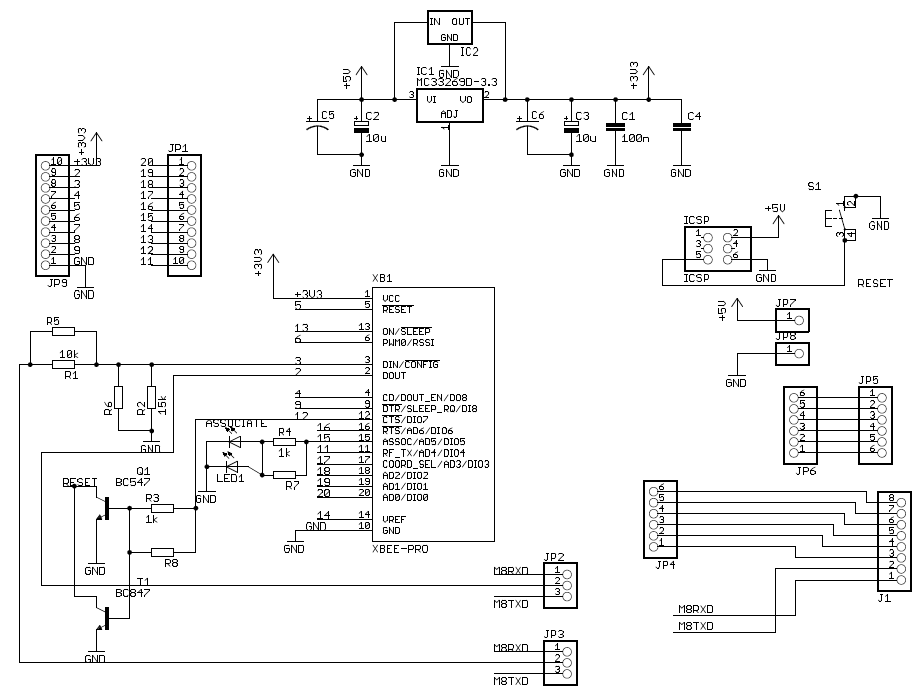
\includegraphics[width=15cm]{xbee_shield.png}
%\caption{Diagram esquemático do módulo shield xBee.}
%\label{fig:xbee}
%\end{figure}

%Todo material do Arduino é disponibilizado pelo fabricante, como a IDE ({\it Integrated Development Environment}) de desenvolvimento, bibliotecas e até mesmo o projeto eletrônico das placas são {\it open source}, ou seja, é permitida a utilização e reprodução sem restrição sobre os direitos autorais dos idealizadores do projeto. Porém o nome Arduino, logotipo e o design gráfico de suas placas são registrados e protegidos por direitos autorais \cite{marcos}.

O projeto Arduino é uma plataforma de hardware e software que facilita desenvolvimento de aplicações que utilizam microcontroladores. O Arduino foi criado com o objetivo de facilitar o aprendizado e possibilitar a prototipação e desenvolvimento de projetos com um custo relativamente baixo, além de não exigir um vasto conhecimento em eletrônica. Estes foram sem dúvida os fatores primordiais para a popularização do Arduino em âmbito mundial, não somente entre os desenvolvedores mais experientes, mas também entre os entusiastas e iniciantes \cite{marcos}.

%Várias pessoas contribuem com a plataforma, seja na construção de novo hardware ou na confecção de novas bibliotecas e materiais de apoio. O Arduino é uma placa muito eficiente e com recursos necessários para a automação de processos de controle e monitoração. Para o desenvolvimento é utilizado o modelo Arduino Uno R3, que é comumente utilizado em projetos básicos. Existem placas ({\it shields}) voltadas para cada tipo de projeto, permitindo controlar um maior número de dispositivos eletrônicos.

%\begin{figure}[!h]
%\centering
%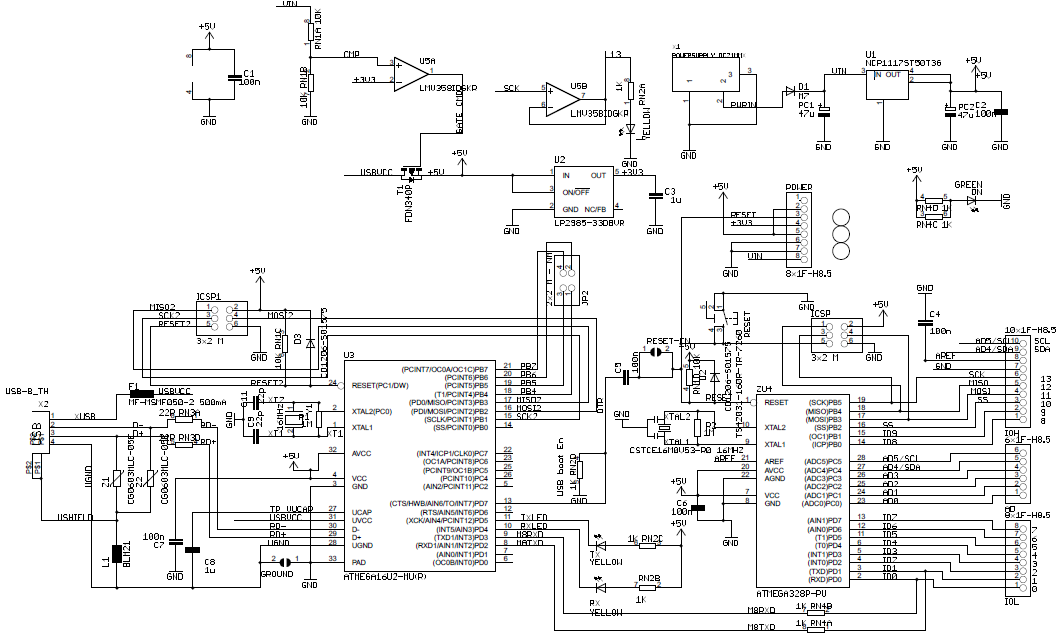
\includegraphics[width=15cm]{arduino.png}
%\caption{Diagram esquemático do módulo Arduino.}
%\label{fig:arduino}
%\end{figure}
%
%O Arduino da Figura \ref{fig:arduino} possui algumas características como:
%
%\begin{itemize}
%\item Microprocessador (responsável pelos cálculos e tomada de decisão);
%\item Memória RAM (utilizada para guardar dados e instruções, volátil);
%\item Memória flash (utilizada para guardar o sotware, não volátil);
%\item Temporizadores (timers);
%\item Contadores;
%\item Clock do sistema.
%\end{itemize}

Muitos microcontroladores possuem memória reduzida e menor poder de processamento, característica da maioria dos sistemas embarcados. O Arduino Uno R3, por exemplo, possui as seguintes especificações:

\begin{itemize}
\item Microcontrolador: ATmega328;
\item Portas Digitais: 14;
\item Portas Analógicas: 6;
\item Memória Flash: 32KB (0.5KB usado no bootloader);
\item SRAM: 2KB;
\item EEPROM: 1KB;
\item Velocidade do Clock: 16MHz.
\end{itemize}

%O circuito interno do Arduino é alimentado com uma tensão contínua de 5V, isto quando é conectado a uma porta USB do computador. Esta conexão fornece a alimentação e também a comunicação de dados. Caso seja necessário é possível utilizar uma fonte de alimentação externa, que forneça uma saída dentre 7,5 V e 12 V com corrente contínua, ou pode ser ligada diretamente na placa utilizando os pinos Vin e GND \cite{marcos}.


%Para o desenvolvimento do projeto foi utilizada plataforma microcontrolada explicada na Seção \ref{aduino}. 
Existem plataformas com diversos objetivos, tais como: placas de comunicação sem fio, sensor de proximidade, emissor de sinal infravermelho, módulo de geolocalização, leitor de cartão por radiofrequência etc.\cite{Hintz:1992:MAP:573880}. Cada um desses módulos tem sua maneira própria de funcionamento e é necessário testar e estudar cada um de maneira individual para melhor fazer uso de suas características.

\begin{figure}[!h]
\centering
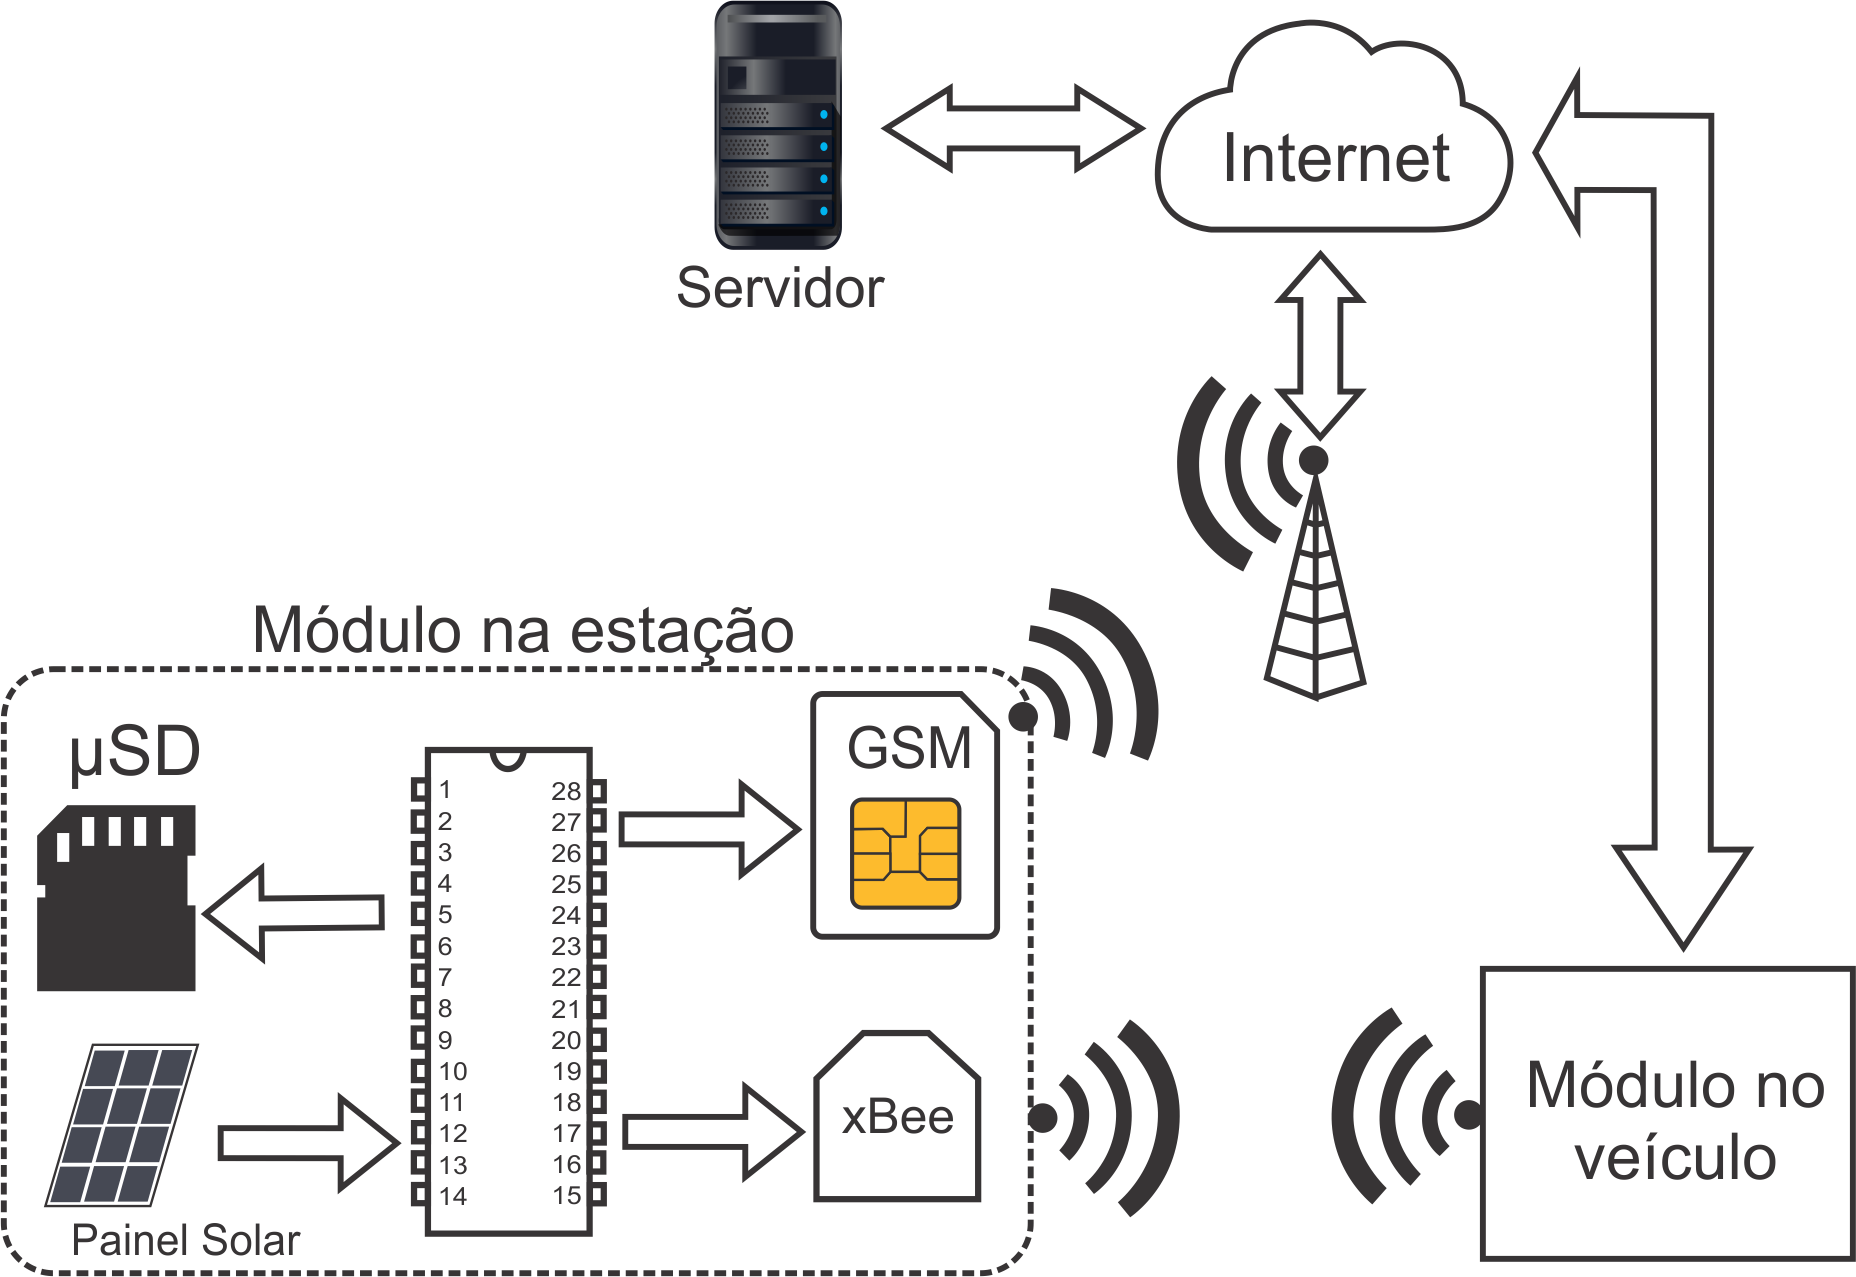
\includegraphics[width=10cm]{ruti2.png}
\caption{Fluxo de dados do projeto.}
\label{fig:modulo_estacao}
\end{figure}

A Figura \ref{fig:modulo_estacao} representa o funcionamento do módulo da estação. O módulo da estação é composto por sub-módulos de:

\begin{itemize}
\item comunicação sem fio xBee \cite{xbee}, que recebe as informações enviadas pelo módulo do veículo;
\item comunicação por rede sem fio de telefonia, que envia os dados colhidos até o servidor;
\item alimentação por energia solar, que abastece o sistema;
\item armazenamento, que grava temporariamente as informações em um cartão microSD;
\item controle geral (microcontrolador), que é responsável por controlar os sub-módulos citados anteriormente.
\end{itemize}

Desse modo, toda vez que um veículo passa pela estação, o módulo recebe as informações do veículo, armazena temporariamente em um cartão microSD e envia através na rede móvel de telefonia para o servidor.

O sub-módulo de comunicação GSM tem foco na rede de dados fornecida pelas operadoras de celulares. O objetivo desse sub-módulo é somente enviar as informações do veículo para um servidor na internet. Essa comunicação é de vital importância para criação de uma base de dados robusta para explorar a análise de tráfego e utilização do transporte público em trabalhos futuros.

Em outro sub-módulo de comunicação será utilizada a comunicação baseado no padrão IEEE 802.15.4, popularmente conhecido com ``ZigBee''. O padrão IEEE 802.15.4 funciona com altas frequências de operação, comparado à sinais mais comuns como rádio frequência, e baixa taxa de transferência de dados. Objetivo é fornecer protocolos seguros e redundantes para manter a integridade dos dados na comunicação. O sub-módulo de comunicação ZigBee será usado na comunicação com a estação ou ponto de ônibus e locais de maior fluxo. Como o sub-módulo GSM possuem latências altas de resposta devido a problemas de infraestrutura, o sub-módulo ZigBee fornece os dados ao módulo na estação e a estação reenvia e ajusta o sincronismo na linha, de modo a permitir que as dados no servidor sejam em tempo real.

Além dos sub-módulos de comunicação externa, o módulo da estação conta com um leitor de cartão de memória, que funcionará como \textit{datalogger}, salvando as informações em caso de falha de comunicação ou outro tipo de falha.

\chapter{Resultados e Discussão}\vskip -12pt

Nesse estudo, foi realizado um teste de comunicação entre dois Arduinos UNO R3, utilizando o módulo xBee. Como o foco deste estudo é somente o módulo de comunicação na estação, ainda não existe um módulo funcional no veículo para transmissão dos dados de maneira adequada. Em substituição aos dados provenientes do veículo, utilizou-se um sensor de temperatura e umidade, modelo DHT11.

Assim, a Figura \ref{fig:umtemp} ilustra o resultado da medições do sensor em período de cinco horas (das 11:00 as 16:00). As leituras foram realizadas no câmpus de Palmas da UFT no dia 16 de agosto de 2018.

\begin{figure}[!h]
\centering
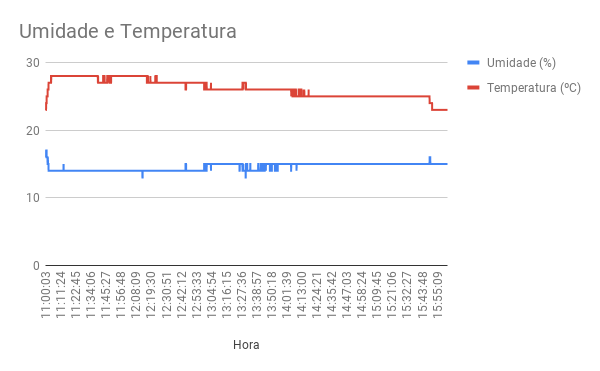
\includegraphics[width=12cm]{Umidade_e_Temperatura_.png}
\caption{Análise da medição realizada durante um período de cinco horas para testar a comunicação entre os módulos.}
\label{fig:umtemp}
\end{figure}

Nesses experimento, o módulo A possui acoplado à ele o módulo xBee e o sensor DHT11, esse módulo transmite as leituras para o módulo B. O módulo B possui a recepção dos dados com outro módulo xBee e por meio da ethernet ele transmite os dados para um \textit{broker}, utilizando o protocolo MQTT (\textit{Message Queuing Telemetry Transport}). Com os dados recebidos no \textit{broker} foi gerado o gráfico da Figura \ref{fig:umtemp}.

\chapter{Considerações Finais}\vskip -12pt

Até o momento foram realizados estudos sobre cada módulo que envolve o projeto. Este estudo demanda bastante tempo, pois é necessário ler a especificação de cada componente e testar suas funcionalidades. Sendo assim, o primeiro módulo testado foi o de comunicação sem fio xBee: um tempo foi dedicado para instalação dos programas necessários para configuração e programação desse módulo específico. Depois, foi feito um projeto de teste para trocar informações entre dois circuitos através desse módulo.

O segundo componente foi o de comunicação por rede móvel de telefonia. Ele tem um microcontrolador um pouco mais robusto, com especificações técnicas mais avançadas e a leitura de seu manual demanda bastante tempo, principalmente se o objetivo é explorar o máximo das suas capacidades. A implementação prática dos testes ainda não aconteceu, pois é preciso de algumas outras ferramentas (como o próprio chip com plano de dados).

%A plataforma de prototipação Arduino \cite{ref:arduino} foi o alvo da maior parcela de estudos. É o Arduino que controlará os módulos específicos e é ele que tem o maior potencial para ser explorado no projeto. Muitas horas de estudo foram dedicadas a testes específicos, envolvendo ferramentas que aumentam o desempenho do microcontrolador, mas demandam mais tempo de desenvolvimento.

%Um dos objetivos da pesquisa inicial para o projeto foi buscar uma alternativa de simplificar o módulo. Para isso, o estudo mais detalhado dos sub-módulos citados no capítulo MATERIAIS E MÉTODOS tiveram como objetivo checar se algum dos sub-módulos era robusto o suficiente para controlar o restante. Apesar de ser uma solução mais elegante, substituir o Arduino como microcontrolador central é uma tarefa bastante trabalhosa. Então foi decidido que as suas características serão exploradas de modo a aperfeiçoar o resultado final.

O próximo passo para o desenvolvimento do projeto é reunir os estudos de cada sub-módulo em um protótipo, que será a primeira versão do sistema implantado nas estações de espera.

%\bibliographystyle{abnt-alf}
\bibliography{bibliografia}


\end{document}

